\documentclass[UTF8]{ctexart}
\usepackage{bookmark}
\usepackage{geometry}
\usepackage{hyperref}
\geometry{a4paper,scale=0.8}
\usepackage{ctex}
\usepackage[style=caspervector,backend=biber,utf8]{biblatex}
\usepackage{booktabs}
\usepackage{array}
\usepackage{fancyhdr}
\pagestyle{fancy}
\fancyhf{}
\renewcommand\footrulewidth{1pt}
\lhead{王铠泽}
\rhead{PB18020766}
\chead{volar@mail.ustc.edu.cn}
\rfoot{中国科学技术大学}
\lfoot{\today}
\usepackage{graphicx}
\usepackage{float}
\usepackage{subfigure}


\begin{document}

	\centering\textbf{\LARGE{计算物理A第六次作业}}
	
	
	王铠泽\qquad PB18020766
	
		
	\section{作业题目}
	
	\begin{itemize}
		\item 对两个函数线型($Gauss$分布和类$Lorentz$型分布),设其一为$p(x)$,另一为
		$F(x)$,用舍选法对$ p(x) $抽样。将计算得到的归一化频数分布直方图与理论曲线$ p(x) $进行
		比较,讨论差异。讨论抽样效率。
		
		本实验中,取$p(x)=\frac{1}{\sqrt{\pi}}e^{-x^2},F(x)=\frac{1}{\sqrt{\pi}}\frac{1}{x^4+1}$。理想效率$\eta=1/Area[F(x)]=\sqrt{\frac{2}{\pi}}\approx0.797885$
		
			\begin{figure}[H]
			\centering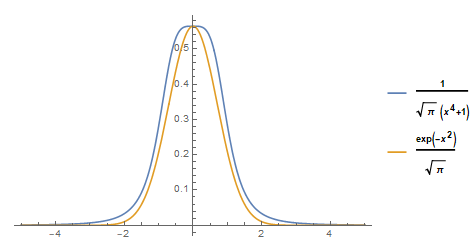
\includegraphics[width=4in]{../figure/func.png}
			\caption{$p(x),F(x)$图例}
			\end{figure}
	\end{itemize}
	
	\section{实现方法}
	
	\begin{itemize}
		\item 舍选法抽样
		
	$F(x)$对应的归一化累计函数为:$$H(x)=G(x)-G(-\infty)$$其中$G(x)$=$\frac{1}{4\pi}[2tan^{-1}(1+\sqrt{2}x)-2tan^{-1}(1-\sqrt{2}x)+ln(\frac{x^2+\sqrt{2}x+1}{x^2-\sqrt{2}x+1})]$,$\lim\limits_{x->\pm\infty}G(x)=\pm\frac{1}{2}$。
	
	\quad 这个函数不易求出反函数,本次实验中采用二分法求得对应$\xi_x$。选定的二分初始区间为
	$[-10,10]$。这个区间对应$H(-10)=0.00015,H(10)=0.99985$,覆盖$99.97\%[0,1]$上随机数。
	
	\begin{figure}[H]
		\centering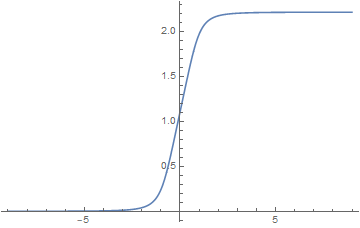
\includegraphics[width=4in]{../figure/F.png}
		\caption{$H(x)$图例}
	\end{figure}
	
	抽样方法:
	生成两个$[0,1]$上随机序列$\xi_1,\xi_2$。在$x$方向上,按$F(x)$分布抽样:$$\xi_1=H(\xi_x)\Rightarrow\xi_x=H^{-1}(\xi_1)$$
	在$y$方向上,按$\frac{1}{F(\xi_x)}$的均匀分布抽样:$$\xi_y=F(\xi_x)\xi_2$$
	比较关系:
	$$\left\{
	\begin{array}{lc}
	\xi_y<p_2(\xi_x)& \Rightarrow accept\\
	\xi_y\geq p_2(\xi_x)& \Rightarrow reject\\
	\end{array}
	\right.
	$$
		
		
		
	
	\end{itemize}
	
	\section{程式说明}
	\begin{itemize}
		\item Rejection.c
		
		该程式使用舍选抽样方法抽取正态分布$\frac{1}{\sqrt{\pi}}e^{-x^2}$分布随机数。包含以下函数:
		
		\subitem double p/F/H (double x)
		
		这三个函数就是前述的$p(x),F(x),H(x)$。
		
		\subitem double root (double xi)
		
		这个函数是通过二分法求解$\xi=H(x)$对应的$x$。其中求解精度$\varepsilon$在函数中为$erf=10^{-4}$。
		
		\item rdm.h
			
		这是一个包含了使用16807产生器生成指定长度的$[0,1]$上均匀分布随机数函数的头文件。
		
		\subitem void rdm(int N,double *x,int method)
		
		该函数将输入的指针$x$对应的长度为$N$的数组用$[0,1]$上的随机数填满。method是关于初始种子的选择。method=0:默认种子;method=1,时间种子。
		
		\item time\_seed.txt
		
		16807产生器抽样时对应的时间种子数据(1个种子)和最终舍选抽样效率(手动加的)。
		
		\item N=10000/100000/1000000.txt
		
		记录了生成的数据文件。
	\end{itemize}
	
	\section{计算结果}

%	\begin{figure}[H]
%	\centering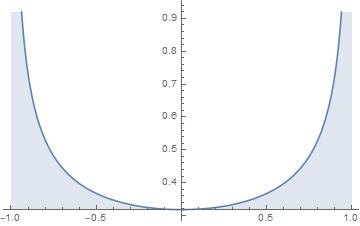
\includegraphics[width=2in]{1.jpg}
%	\caption{something}\label{fig:1}
%	\end{figure}
	
%	\begin{figure}[H]
%		\centering  %图片全局居中
%		\subfigure[直接抽样$x-y$平面分布]{
%			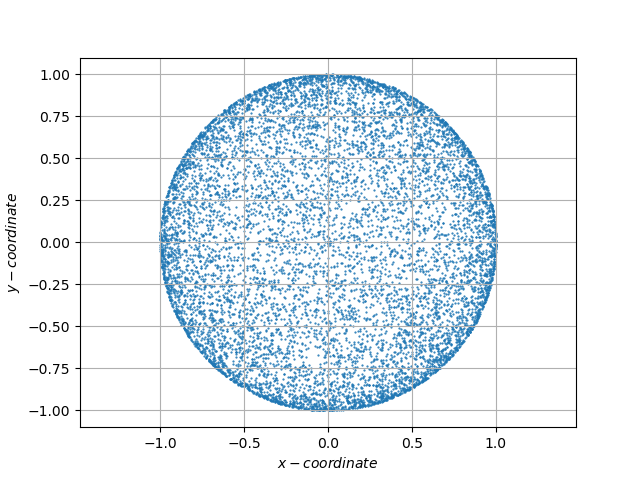
\includegraphics[width=0.45\textwidth]{../x-y.png}}
%		\subfigure[$Marsaglia$抽样$x-y$平面分布]{
%			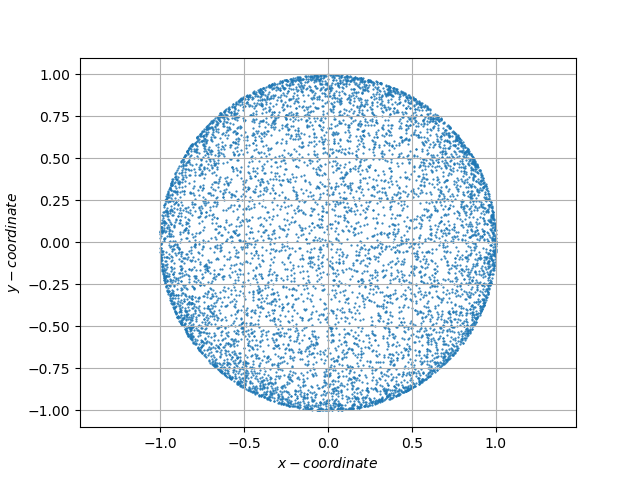
\includegraphics[width=0.45\textwidth]{../M-x-y.png}}
%		\subfigure[直接抽样$x-z$平面分布]{
%			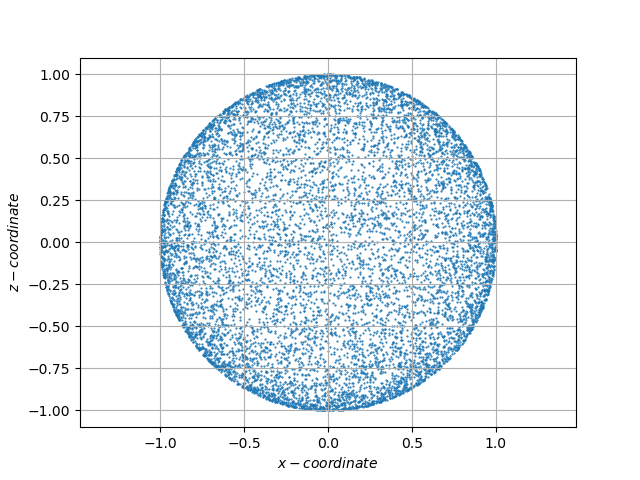
\includegraphics[width=0.45\textwidth]{../x-z.png}}
%		\subfigure[$Marsaglia$抽样$x-z$平面分布]{
%			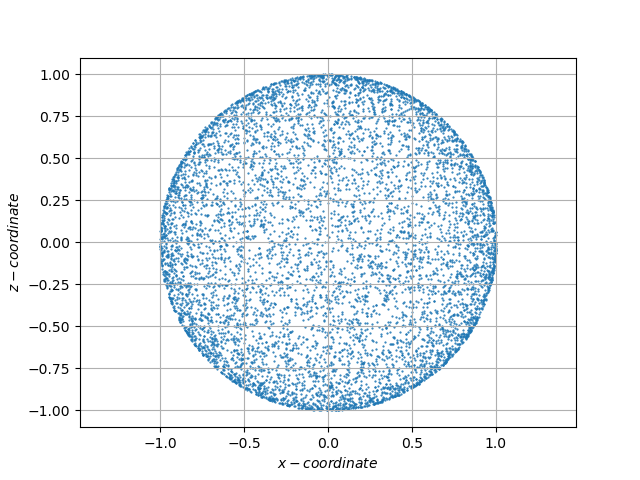
\includegraphics[width=0.45\textwidth]{../M-x-z.png}}
%		\caption{抽样分布}
%		\label{N}
%	\end{figure}
%	
	
	\begin{flushleft}
		
	分别在总点数$N=10000,10000,100000$下得到归一化直方图。默认参数$bin=500$,红色虚线为理想分布。
	\end{flushleft}
	
		\begin{figure}[H]
			\centering  %图片全局居中
			\subfigure[$N=10000$,$\eta=0.793200$]{
				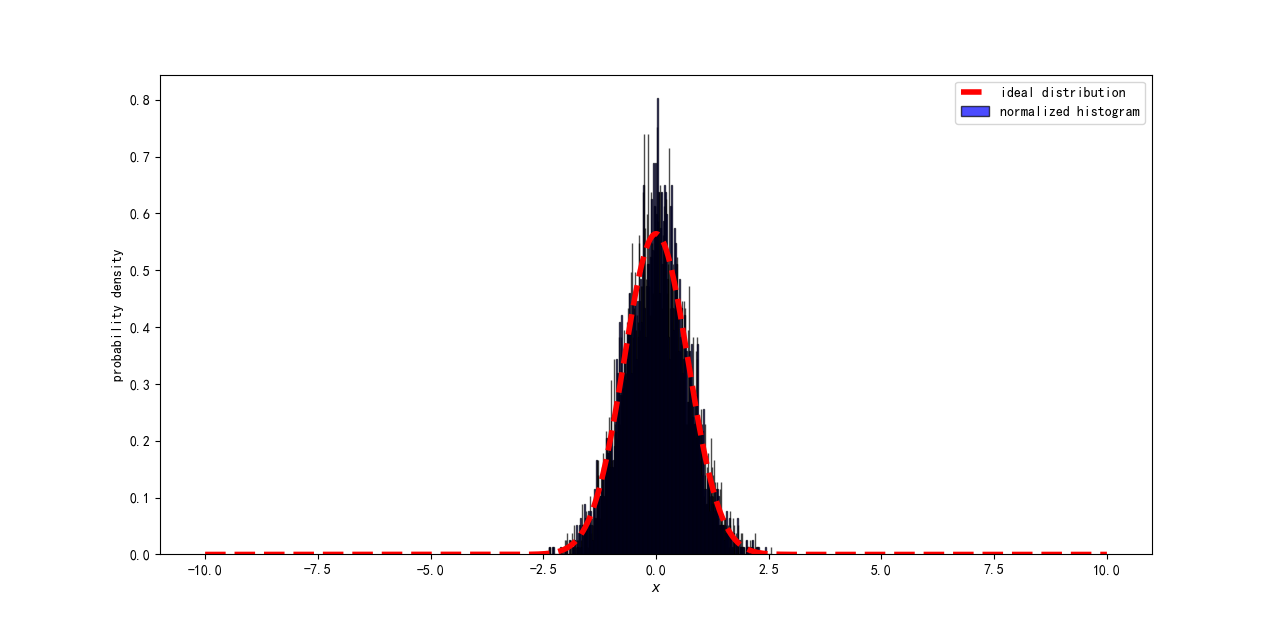
\includegraphics[width=0.6\textwidth]{../figure/N=10000.png}}
			\subfigure[$N=100000$,$\eta=0.798740$]{
				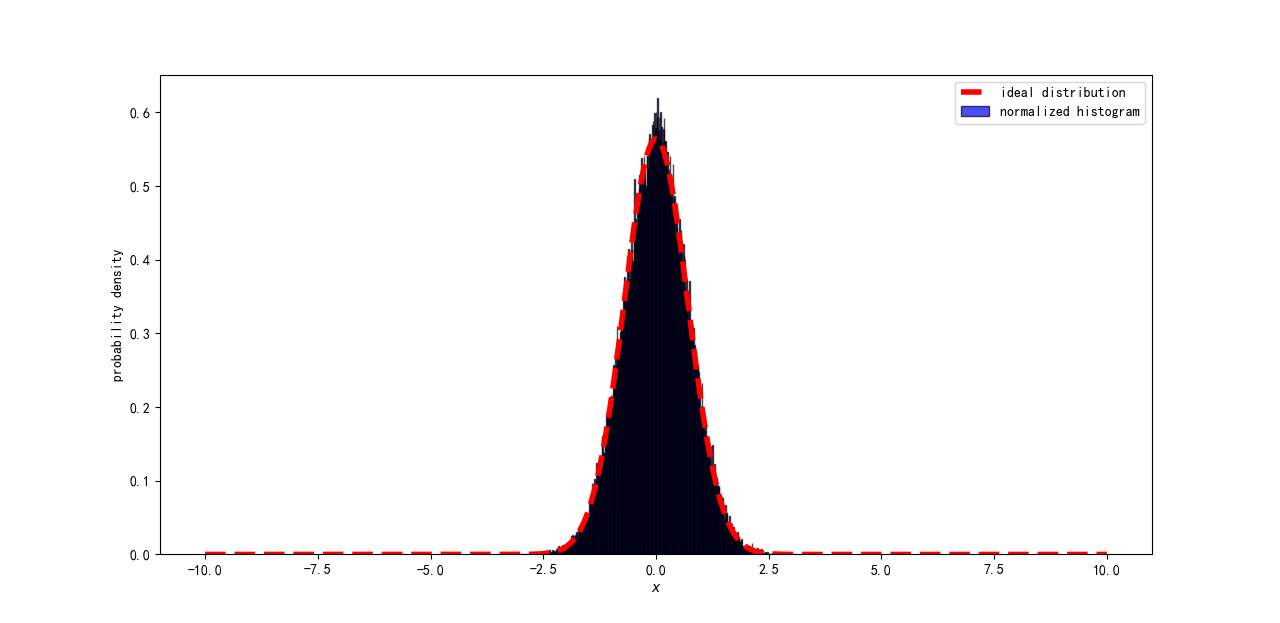
\includegraphics[width=0.6\textwidth]{../figure/N=100000.png}}
			\subfigure[$N=1000000$,$\eta=0.798477$]{
				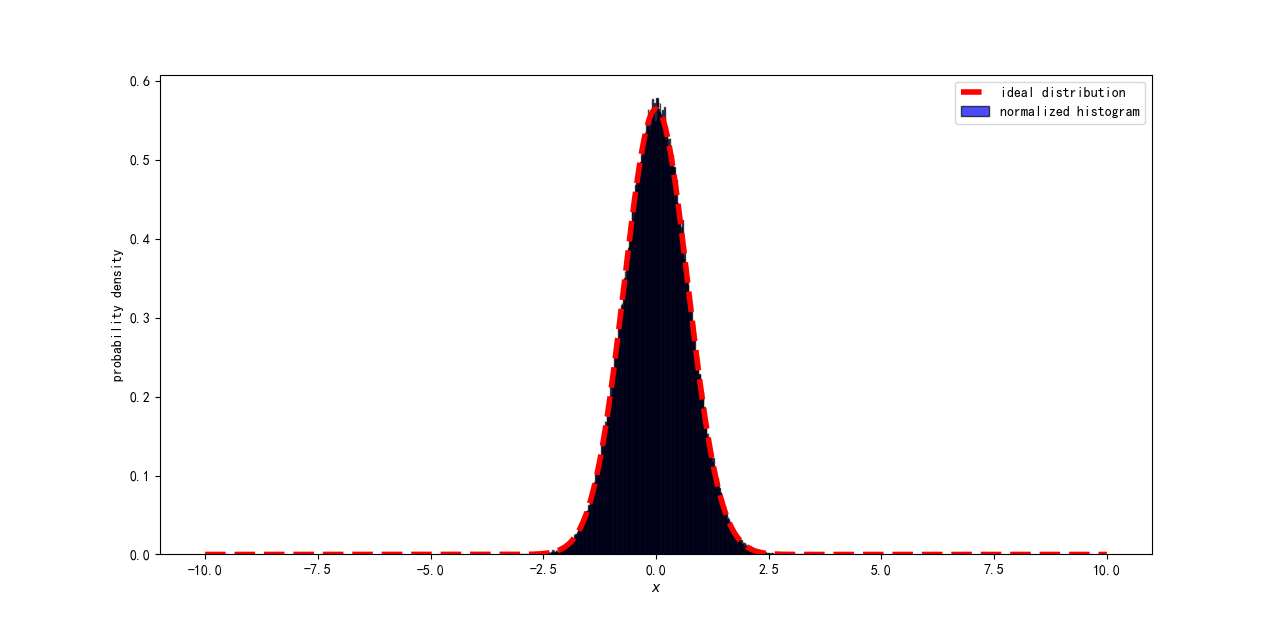
\includegraphics[width=0.6\textwidth]{../figure/N=1000000.png}}
			\caption{归一化直方图}
		\end{figure}
\begin{flushleft}
		可见,随着$N$增大,频数分布逐渐趋于理想分布。
\end{flushleft}

	\clearpage
	\section{总结}
	\begin{itemize}
		\item 本次实验采用舍选法,利用和$Guass$函数形状类似的$Lorentz$型函数作为比较函数抽样,提供了又一种正态抽样的方法。
		\item 为了提高运算速度,应该考虑如何对$F(x)$进行抽样,寻找比二分法求逆更有效率方式。
	\end{itemize}
	\clearpage
\end{document}